%git 
% Copyright 2017 Markus Borg, Lund University
%
% This work is licensed under a Creative Commons Attribution-ShareAlike 4.0 International License.
% See http://creativecommons.org/licenses/by-sa/4.0/
%
% The dodument is based on a LaTeX template developed by Jean-Philippe Eisenbarth
% https://github.com/jpeisenbarth/SRS-Tex
%
\documentclass{scrreprt}
\usepackage{graphicx}
\usepackage{listings}
\usepackage{underscore}
\usepackage[bookmarks=true]{hyperref}
\usepackage[utf8]{inputenc}
\usepackage[english]{babel}
\hypersetup{
    bookmarks=false,    % show bookmarks bar?
    pdftitle={Lab 2},    % title
    pdfauthor={Markus Borg},                     % author
    pdfsubject={TeX and LaTeX},                        % subject of the document
    pdfkeywords={TeX, LaTeX, graphics, images}, % list of keywords
    colorlinks=true,       % false: boxed links; true: colored links
    linkcolor=blue,       % color of internal links
    citecolor=black,       % color of links to bibliography
    filecolor=black,        % color of file links
    urlcolor=purple,        % color of external links
    linktoc=page            % only page is linked
}%
\def\myversion{1.2 }
\date{}
%\title
\usepackage{hyperref}
\begin{document}

\begin{flushright}
    \rule{16cm}{5pt}\vskip1cm
    \begin{bfseries}
    	\LARGE{ETSA02-ADM-LAB2}\\
    	\vspace{1.5cm}
        \Huge{Lab 2}\\
        \vspace{0.5cm}
        Object-oriented design\\
        \vspace{0.5cm}
        and unit testing\\
        \vspace{1.5cm}
        \LARGE{Version \myversion approved}\\
        \vspace{1.5cm}
        Prepared by Markus Borg\\
        %\vspace{1.5cm}
        Dept. of Computer Science, Lund University\\
        \vspace{1.5cm}
        \today\\
    \end{bfseries}
\end{flushright}

%\tableofcontents

\chapter*{Revision History}

\begin{center}
    \begin{tabular}{|c|c|c|c|}
        \hline
	    Name & Date & Reason For Changes & Version\\
        \hline
	    Markus Borg & 2017-12-11 & Initial draft. & 0.1\\
        \hline
        Markus Borg & 2018-03-21 & Changed to refactoring+unit testing. & 0.2\\
        \hline
        Markus Borg & 2018-03-21 & Complete draft. & 0.3\\
        \hline
        Markus Borg & 2018-03-22 & Updated after internal review. & 0.4\\
        \hline
        Markus Borg & 2018-03-25 & Clarified after more internal review. & 0.5\\
        \hline
        Markus Borg & 2018-03-26 & Version ready for lab. & 1.0\\
        \hline
        Markus Borg & 2019-03-30 & Updated to use the introsofteng-botexample repo. & 1.1\\
        \hline
        Markus Borg & 2019-04-05 & Clarified attributes of the class MovementSystem. & 1.2\\
        \hline
    \end{tabular}
\end{center}

\chapter{Introduction}
Lab 2 will inspire you to organize your robot implementation according to a a proper object-oriented design. Furthermore, the lab will help you get started with unit testing using the JUnit framework. More specifically, Lab 2 covers:

\begin{itemize}
\item Program comprehension, i.e., reading code of a somewhat more advanced robot.
\item Reading a UML class diagram.
\item Refactoring source code.
\item Working with JUnit in Eclipse.
\end{itemize}

\chapter{Before the lab}
To save time during the lab session, please read through this section and follow the instructions. Also, unless you are already familiar with it, please read how the Robocode coordinate system works. One source to understand navigation in Robocode is this link: http://mark.random-article.com/weber/java/robocode/lesson4.html

Wikipedia is a great source to read up on software engineering topics. Software engineers appear to carefully monitor and describe their work practices. Perhaps they take pride in describing what they do for the masses? Good for us, Wikipedia (at least in English) is a free and often accurate source of software engineering knowledge. Besides, reading from other sources than the course book is a good idea.

Prior to the lab, please browse the following Wikipedia articles:
\begin{itemize}
\item Object oriented programming (skip ``History'' and onwards)\\-- https://en.wikipedia.org/wiki/Object-oriented_programming)
\item Class diagram\\-- https://en.wikipedia.org/wiki/Class_diagram
\item Code refactoring\\-- https://en.wikipedia.org/wiki/Code_refactoring
\item Unit testing\\-- https://en.wikipedia.org/wiki/Unit_testing
\end{itemize}

The course material is maintained under an open source license on GitHub. Almost everything we will use in the course is stored in one of the following repositories:
\begin{itemize}
\item https://github.com/lunduniversity/introsofteng -- This is the backbone of the course, containing the project instructions, lectures, lab instructions like this document, and exercises.
\item https://github.com/lunduniversity/introsofteng-botexample -- This is the skeleton of Basic Melee Bot that you will implement in Lab~2. To support you, the repository contains a suite of unit test cases. In Lab~3, you will implement automated system test cases for Basic Melee Bot. Furthermore, the repository contains all dependencies needed for the project. Your group is encouraged to use this repository as a template when creating the robot for the project.
\end{itemize}

You are all welcome to contribute to the repositories if you find errors or obvious improvements. Once you are comfortable with git, you are most welcome to create ``pull requests'' to improve the course material, e.g., clarifying descriptions or correcting typos!

To ensure that you get the correct version of the source code for Lab~2, we recommend that you download the latest \textit{release}, i.e., a container of one or more assets, associated to a git annotated tag. GitHub uses releases to package software versions to users. Open a web browser and go to https://github.com/lunduniversity/introsofteng-botexample. Figure~\ref{fig:github-release} shows where you find the releases created for this repository -- click on it. Figure~\ref{fig:github-zip} should appear and list all available releases. For Lab~2, download the source code for v1.1 as a zip file as indicated by the arrow.

\begin{figure}
\centering
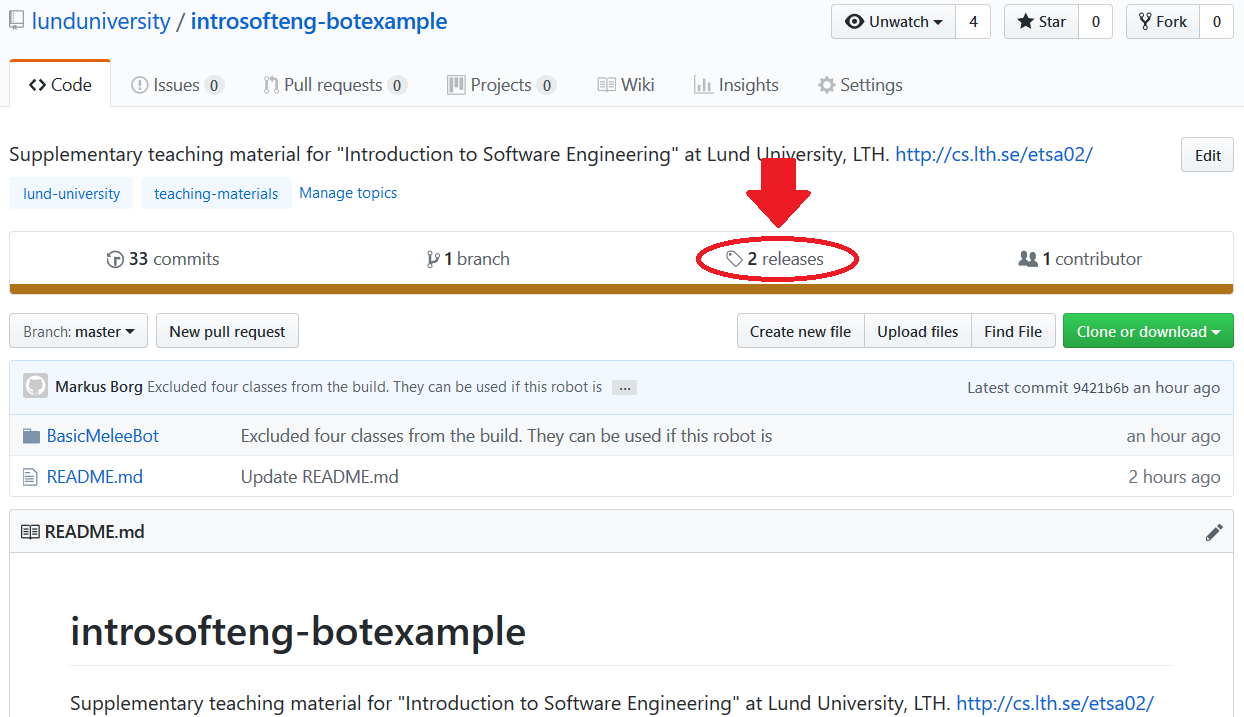
\includegraphics[width=0.99\textwidth]{figures/GitHub-release.png}
\caption{Finding the releases of introsofteng-botexample on GitHub.}
\label{fig:github-release}
\end{figure}

\begin{figure}
\centering
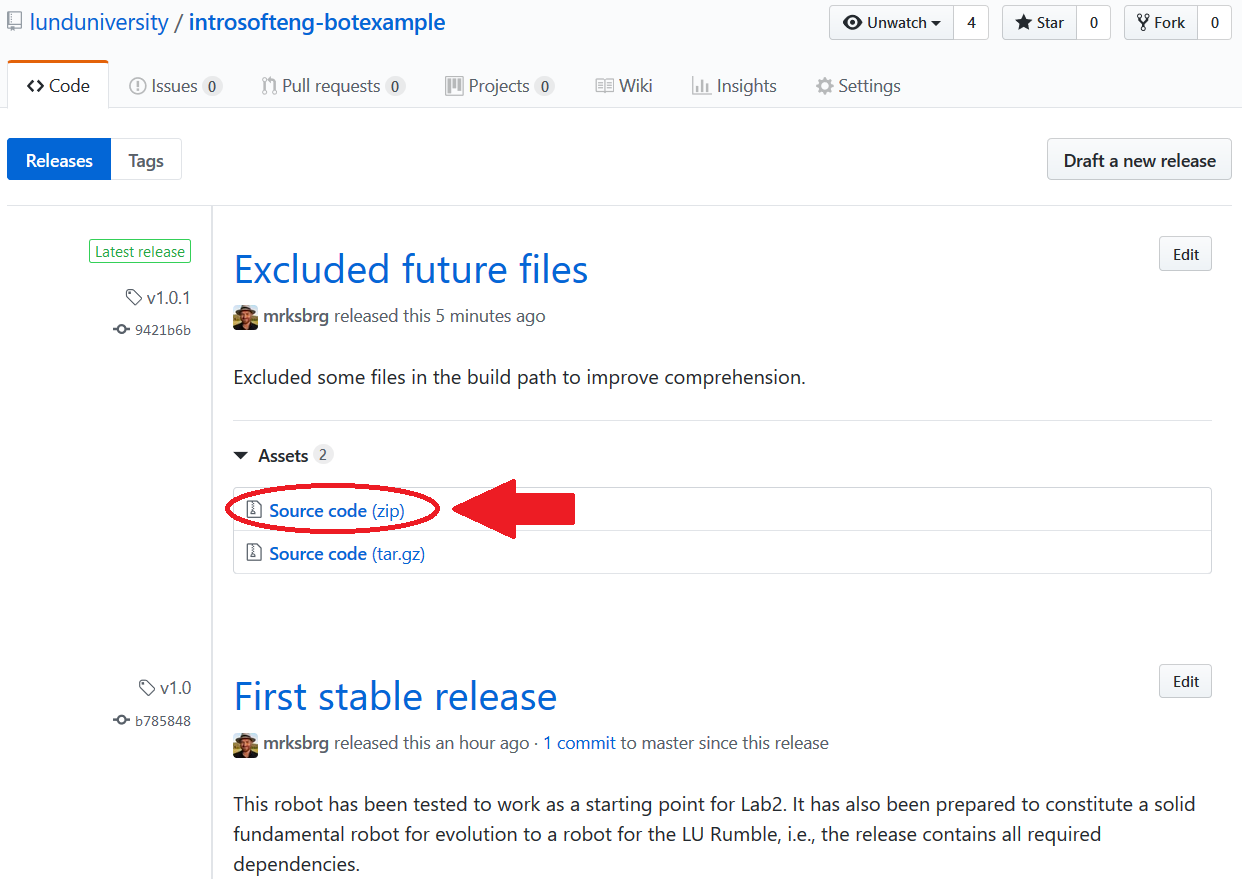
\includegraphics[width=0.99\textwidth]{figures/GitHub-zip.png}
\caption{Downloading the source code corresponding to a release on GitHub. The arrow shows the zip archive. Note: you should download the latest release, currently 1.1.}
\label{fig:github-zip}
\end{figure}

\chapter{At the lab}
The first thing you need to do is to import the Lab~2 source code, then it is time to get started with automated testing using JUnit. Follow the steps below.\\

\textbf{Import the source code:}
\begin{enumerate}
\item Start Eclipse.
\item Run ``Import...'' from the File menu.
\item Under ``General'' choose ``Projects from Folder or Archive'' and click ``Next''.
\item Import the project as shown in Figure~\ref{fig:eclipse-import}. First, click ``Archive..'' and select the zip file you downloaded. Second, select only the checkbox for the Eclipse project. Third, click ``Finish''.
\item Verify that the content in the Package Explorer resembles Figure~\ref{fig:afterImport}.
\end{enumerate}

\textbf{Configure and run the JUnit unit test suite:}
\begin{enumerate}
\item Right click on BMBUnitTestSuite.java in the Package Explorer. Select ``Run Configurations...'' under ``Run As''.
\item In the dialog that appears, create a new JUnit configuration. Enter the information presented in Figure~\ref{fig:runConfig}.
\item Click ``Run''. All units tests in the test suite shall now run. All of them are supposed to fail!
\end{enumerate}

\begin{figure}
\centering
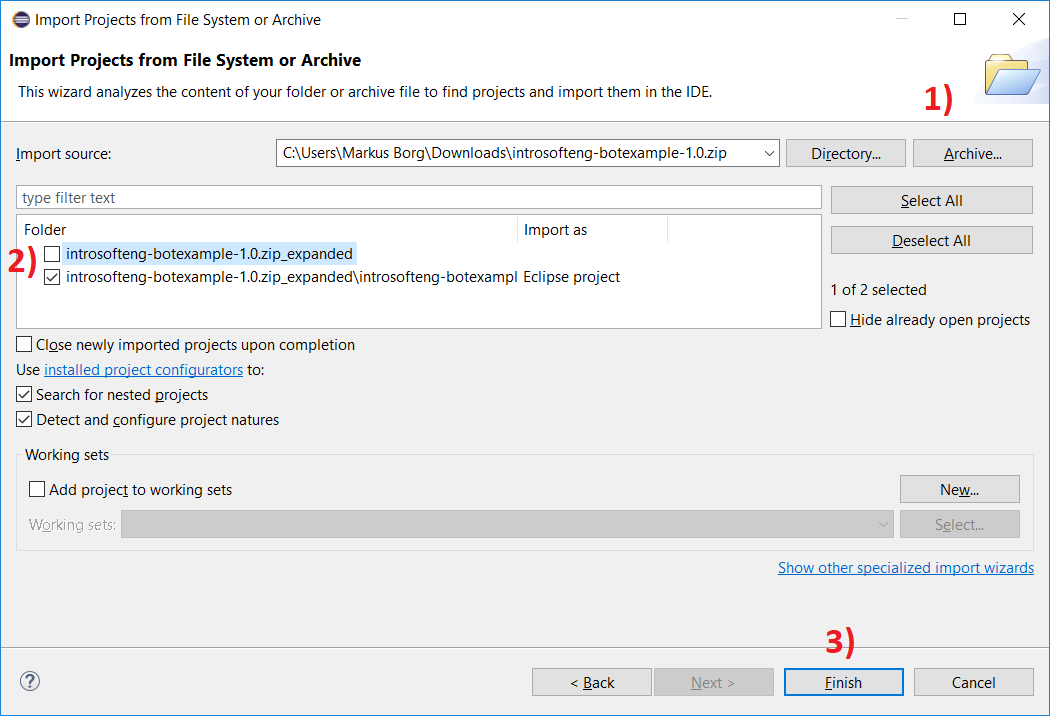
\includegraphics[width=0.99\textwidth]{figures/Eclipse-import.png}
\caption{Downloading the source code corresponding to a release on GitHub. The arrow shows the zip archive.}
\label{fig:eclipse-import}
\end{figure}

\begin{figure}
\centering
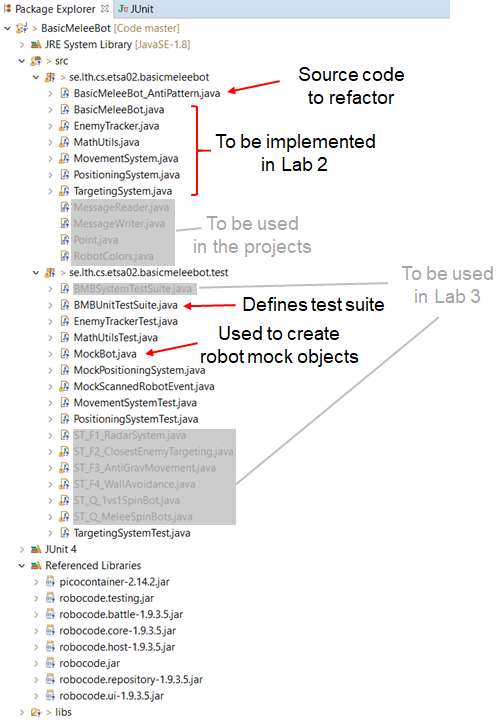
\includegraphics[width=0.85\textwidth]{figures/packageExplorerAfterImport.png}
\caption{The Package Explorer in Eclipse after importing the source code from introsofteng-examplebot.}
\label{fig:afterImport}
\end{figure}

\begin{figure}
\centering
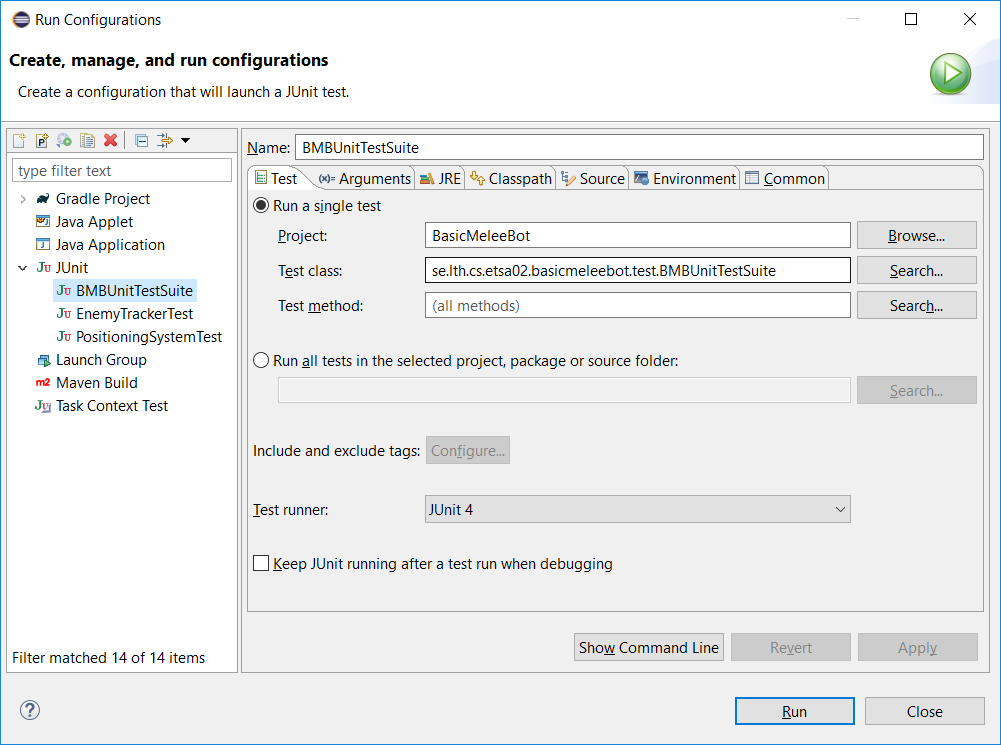
\includegraphics[width=0.99\textwidth]{figures/JUnit-runConfig.png}
\caption{Creating a new JUnit run configuration for BMBUnitTestSuite.}
\label{fig:runConfig}
\end{figure}

\newpage

\textbf{Complete the refactoring task:}
\begin{enumerate}
\item First, you should study the implementation of the robot in ``BasicMeleeBot_AntiPattern''. The robot implements ``anti gravity movement'', i.e., it moves away from other robots. 
\item Try the robot in Robocode to verify the anti gravity movement. For Robocode to find Basic Melee Bot, you first need to set the path to the root directory of the BasicMeleeBot project in the ``Development Options'' under ``Options$\rightarrow$Preferences'' in Robocode. Revisit the instructions for Lab~1 if you do not remember how to do this.
\item BasicMeleeBot_AntiPattern does not comply with good object oriented design practices, instead all functionality is collected in one big class. A modular robot design would greatly increase the evolvability of the product. Figure~\ref{fig:classDiagram} shows a more feasible object oriented design. Perhaps you can use something similar in your project?
\item Your task is now to refactor BasicMeleeBot_AntiPattern into the structure presented in the provided class diagram. BasicMeleeBot.java is already implemented for you, but you should complete the missing code in the other classes. A suggested implementation order is: 1) MathUtils, 2) PositioningSystem, 3) EnemyTracker, 4) TargetingSystem, and 5) MovementSystem. The unit tests are there to guide you in the process. Study the test cases to understand the intention behind the different methods. Most importantly, run them frequently to verify that you are on the right track -- when all test cases are green, you have completed Lab 2!
\begin{center}
\textbf{------ REACH THIS POINT TO PASS LAB 2! ------}
\end{center}
\item If time permits during Lab~2, uncomment the code snippet for ``wall avoidance'' in MovementSystem.java and move it according to the instructions. If you did not reach this point during the lab session, please do it before Lab~3 -- it is required to proceed with the automated system testing. Start Robocode and verify that Basic Melee Bot does not end up in any wall. \\\\If wall avoidance does not work, please pay attention to the red arrow in Figure~\ref{fig:classDiagram}. If you have copied the entire code snippet from the \#\#\#\#\#\#\# MOVEMENT \#\#\#\#\#\#\# section in BasicMeleeBot\_AntiPattern, then you have declared two new local variables with the same names in MovementSystem, i.e., these variables now \textit{shadow} the attributes -- make sure the update() method in MovementSystem indeed updates the attributes, not any local variables.
\end{enumerate}

\begin{figure}
\centering
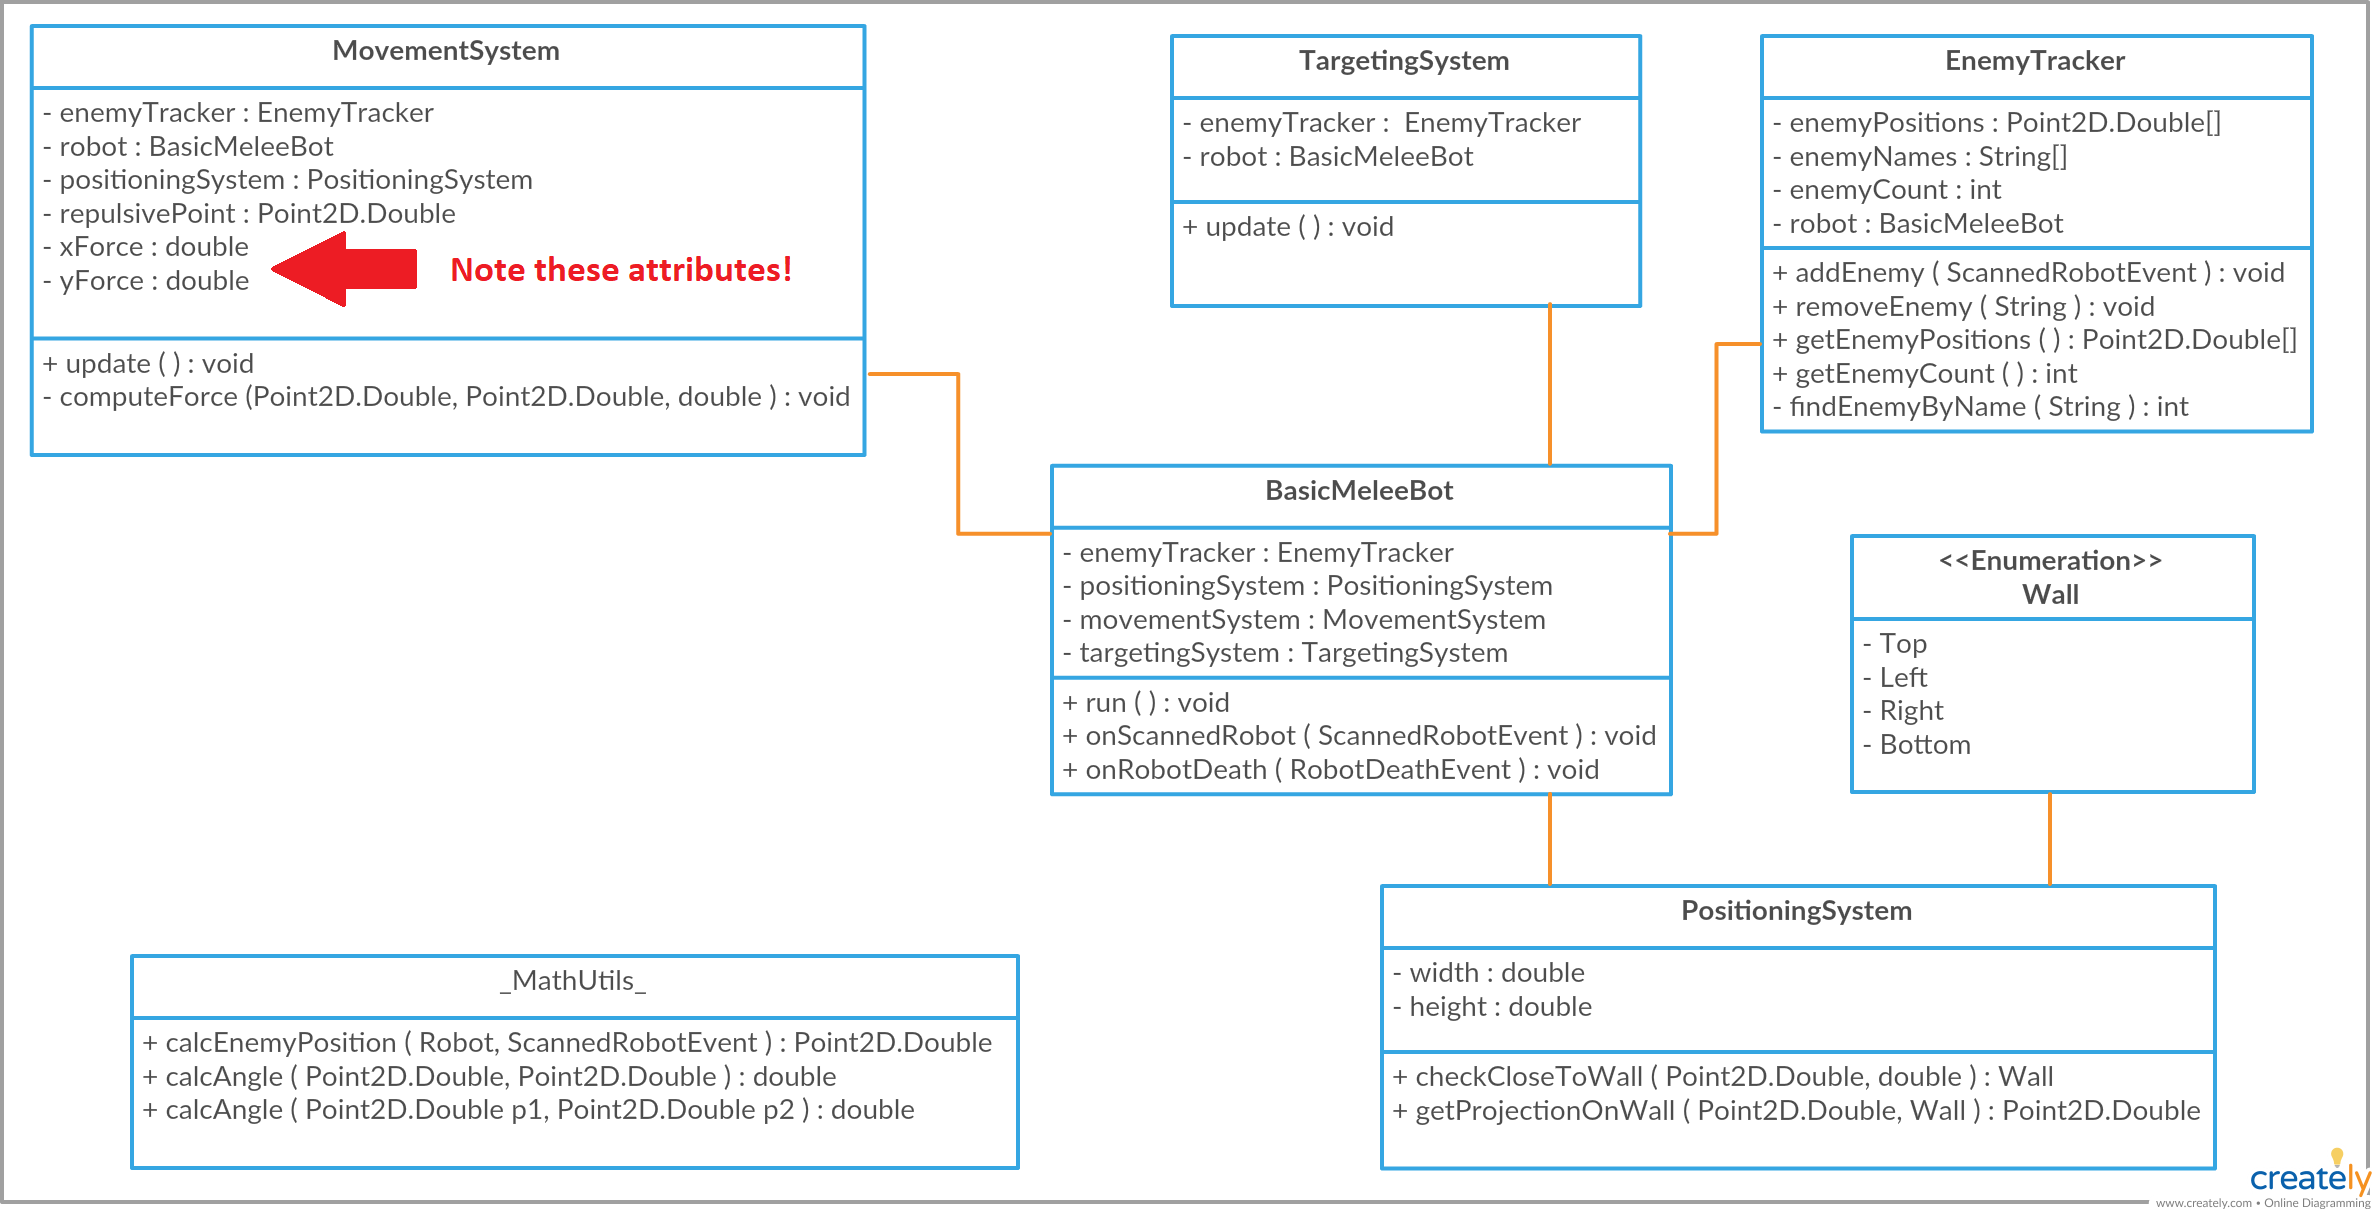
\includegraphics[width=1.1\textwidth]{figures/BasicMeleeBotClassDiagram.png}
\caption{BasicMeleeBot class diagram. Note that MathUtils is a static class. Also note the two attributes xForce and yForce in MovementSystem -- there is a corresponding instruction in step 5 in the refactoring task.}
\label{fig:classDiagram}
\end{figure}

\newpage

\chapter{After the lab}
During the lab you have practiced several fairly advanced software engineering practices at the same time. You have refactored source code into a modular object-oriented design, guided by a UML class diagram, while adhering to a test-driven development approach supported by automated unit testing. Well done!

When your project releases software, you are supposed to provide the regulatory body with a UML class diagram and source code complemented with a suite of JUnit test cases. Note that the group purchasing your robot shall not receive anything of this, they get only the requirements specification, the test specification, and the executable robot as a .jar file.

We recommend that the group helps the software architect to maintain a class diagram of the most recent robot design. Also, the group shall together maintain a JUnit test suite as an approach to detect bugs early -- you should obviously run your test suite frequently. In industry, developers are typically responsible for writing unit tests for all their source code -- this is generally a good practice. The test cases would then run every time there is a commit as part of a continuous integration pipeline.

\end{document}
